\documentclass[dvisvgm,multi=true]{standalone}
\usepackage{mathmlcoresvg}
\begin{document}
%<figcaption><span>Figure 24: </span>Box model for the <code>mmultiscripts</code> element</figcaption>
  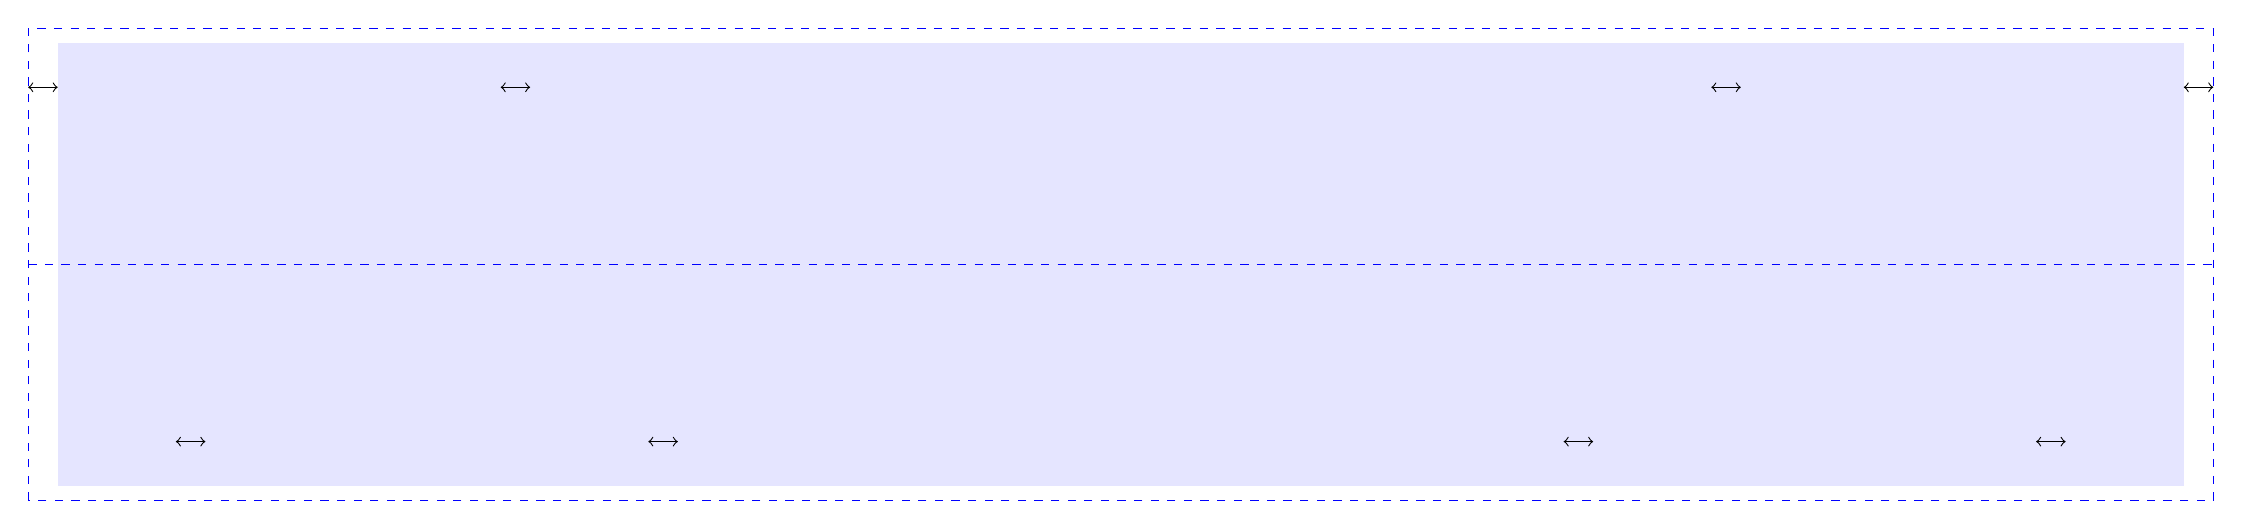
\begin{tikzpicture}[yscale=-.75,xscale=.75]

  \fill[blue!10](-15.5,3.75) rectangle (20.5,-3.75);

  \draw[dashed,blue](-16,4) rectangle(21,-4)
  (-16,0)--(21,0);

  \MathMLBox{0}{0}{1}{1}{red};

  \MathMLBox{5}{-3}{1.5}{.5}{green};
  \draw[<->] (12.5,-3) -- (13,-3);

  \MathMLBox{5}{3}{1}{.5}{green};
  \draw[<->] (10,3) -- (10.5,3);

  \begin{scope}[shift={(8,0)}]
  \MathMLBox{5}{-3}{1.5}{.5}{green};
  \draw[<->] (12.5,-3) -- (13,-3);

  \MathMLBox{5}{3}{1}{.5}{green};
  \draw[<->] (10,3) -- (10.5,3);
  \end{scope}

  \begin{scope}[shift={(-12.5,0)}]
  \MathMLBox{5}{-3}{1.5}{.5}{green};
  \draw[<->] (4.5,-3) -- (5,-3);

  \begin{scope}[shift={(2.5,0)}]
  \MathMLBox{5}{3}{1}{.5}{green};
  \draw[<->] (4.5,3) -- (5,3);
  \end{scope}
  \end{scope}

  \begin{scope}[shift={(-20.5,0)}]
  \MathMLBox{5}{-3}{1.5}{.5}{green};
  \draw[<->] (4.5,-3) -- (5,-3);

  \begin{scope}[shift={(2.5,0)}]
  \MathMLBox{5}{3}{1}{.5}{green};
  \draw[<->] (4.5,3) -- (5,3);
  \end{scope}
  \end{scope}

\end{tikzpicture}

\end{document}
